\begin{figure}[htbp]
    \centering
    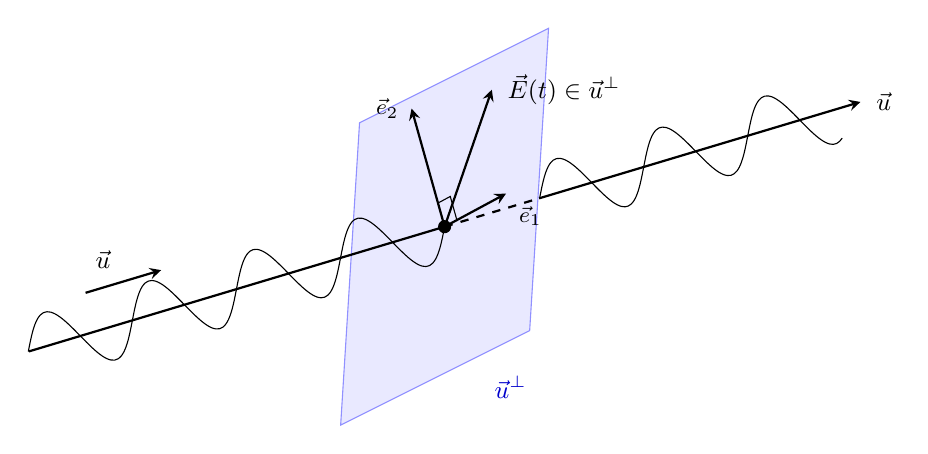
\begin{tikzpicture}[scale=1.2, >=stealth]
        % --- Points de référence de l'axe du rayon u (incliné montant) ---
        \coordinate (O)     at (0, 0);               % Centre / intersection
        \coordinate (Left)  at (-4.4, -1.32);        % Origine gauche basse
        \coordinate (Mid)   at (1.0, 0.3);           % Fin de la zone cachée
        \coordinate (Right) at (4.4, 1.32);          % Arrivée droite haute

        % ==============================================================
        % 1. PLAN ORTHOGONAL u^\bot (davantage incliné, teinté bleu)
        % ==============================================================
        % Sommets du parallélogramme basculé
        \coordinate (P1) at (-1.1, -2.1);
        \coordinate (P2) at (0.9, -1.1);
        \coordinate (P3) at (1.1, 2.1);
        \coordinate (P4) at (-0.9, 1.1);

        \filldraw[fill=blue!10, draw=blue!50, thin, opacity=0.85] 
            (P1) -- (P2) -- (P3) -- (P4) -- cycle;

        % Label du plan u^\bot
        \node[blue!80!black, font=\small] at (0.7, -1.7) {$\vec{u}^\perp$};

        % ==============================================================
        % 2. AXE DU RAYON LUMINEUX (Incliné montant vers la droite)
        % ==============================================================
        % Segment amont
        \draw[thick] (Left) -- (O);
        
        % Traversée immédiate après le centre (atténuée/pointillée)
        \draw[thick, dashed] (O) -- (Mid);
        
        % Segment aval émergeant
        \draw[thick, ->] (Mid) -- (Right) node[right=2pt, font=\small] {$\vec{u}$};

        % Flèche et label du vecteur u au départ
        \draw[thick, ->] (-3.8, -0.7) -- (-3.0, -0.46) 
            node[midway, above left=1pt, font=\small] {$\vec{u}$};

        % ==============================================================
        % 3. ONDE SINUSOÏDALE (le long de l'axe incliné)
        % ==============================================================
        % Rotation locale de l'onde pour suivre la pente (environ 16.7 degrés)
        \begin{scope}[rotate around={16.7:(O)}]
            % Onde amont (x de -4.6 à 0)
            \draw[domain=-4.6:0, samples=120, smooth, variable=\x, thin, black] 
                plot ({\x}, {0.35*sin((\x+4.6)*360/1.15)});

            % Onde aval (x de 1.05 à 4.3)
            \draw[domain=1.05:4.3, samples=90, smooth, variable=\x, thin, black] 
                plot ({\x}, {0.35*sin((\x-1.05)*360/1.15)});
        \end{scope}

        % ==============================================================
        % 4. BASE ORTHOGONALE ET VECTEUR E(t) DANS LE PLAN
        % ==============================================================
        % Vecteur e2 (direction haute du plan)
        \draw[thick, ->] (O) -- (-0.35, 1.25) node[left=1pt, font=\footnotesize] {$\vec{e}_2$};
        
        % Vecteur e1 (oblique, fuite vers la droite dans le plan)
        \draw[thick, ->] (O) -- (0.65, 0.35) node[below right=1pt, font=\footnotesize] {$\vec{e}_1$};

        % Symbole d'angle droit entre e1 et e2
        \draw[thin] (-0.07, 0.25) -- (0.06, 0.32) -- (0.13, 0.07);

        % Vecteur champ électrique E(t)
        \draw[thick, ->, black] (O) -- (0.5, 1.45) 
            node[right=2pt, font=\small] {$\vec{E}(t) \in \vec{u}^\perp$};

        % Point central d'impact O
        \filldraw[fill=black] (O) circle (1.8pt);
    \end{tikzpicture}
    \caption{Propagation libre le long de $\vec{u}$ et confinement de l'oscillation transverse $\vec{E}(t)$ dans le plan orthogonal $\vec{u}^\perp = \mathrm{Vect}(\vec{e}_1, \vec{e}_2)$.}
    \label{fig:onde_transverse_inclinee}
\end{figure}